\thispagestyle{timhieukhoahocnone}
\pagestyle{timhieukhoahoc}
\everymath{\color{timhieukhoahoc}}
\blfootnote{\color{timhieukhoahoc}$^1$Hà Nội.}
\graphicspath{{../timhieukhoahoc/pic2/}}
\begingroup
\AddToShipoutPicture*{\put(0,616){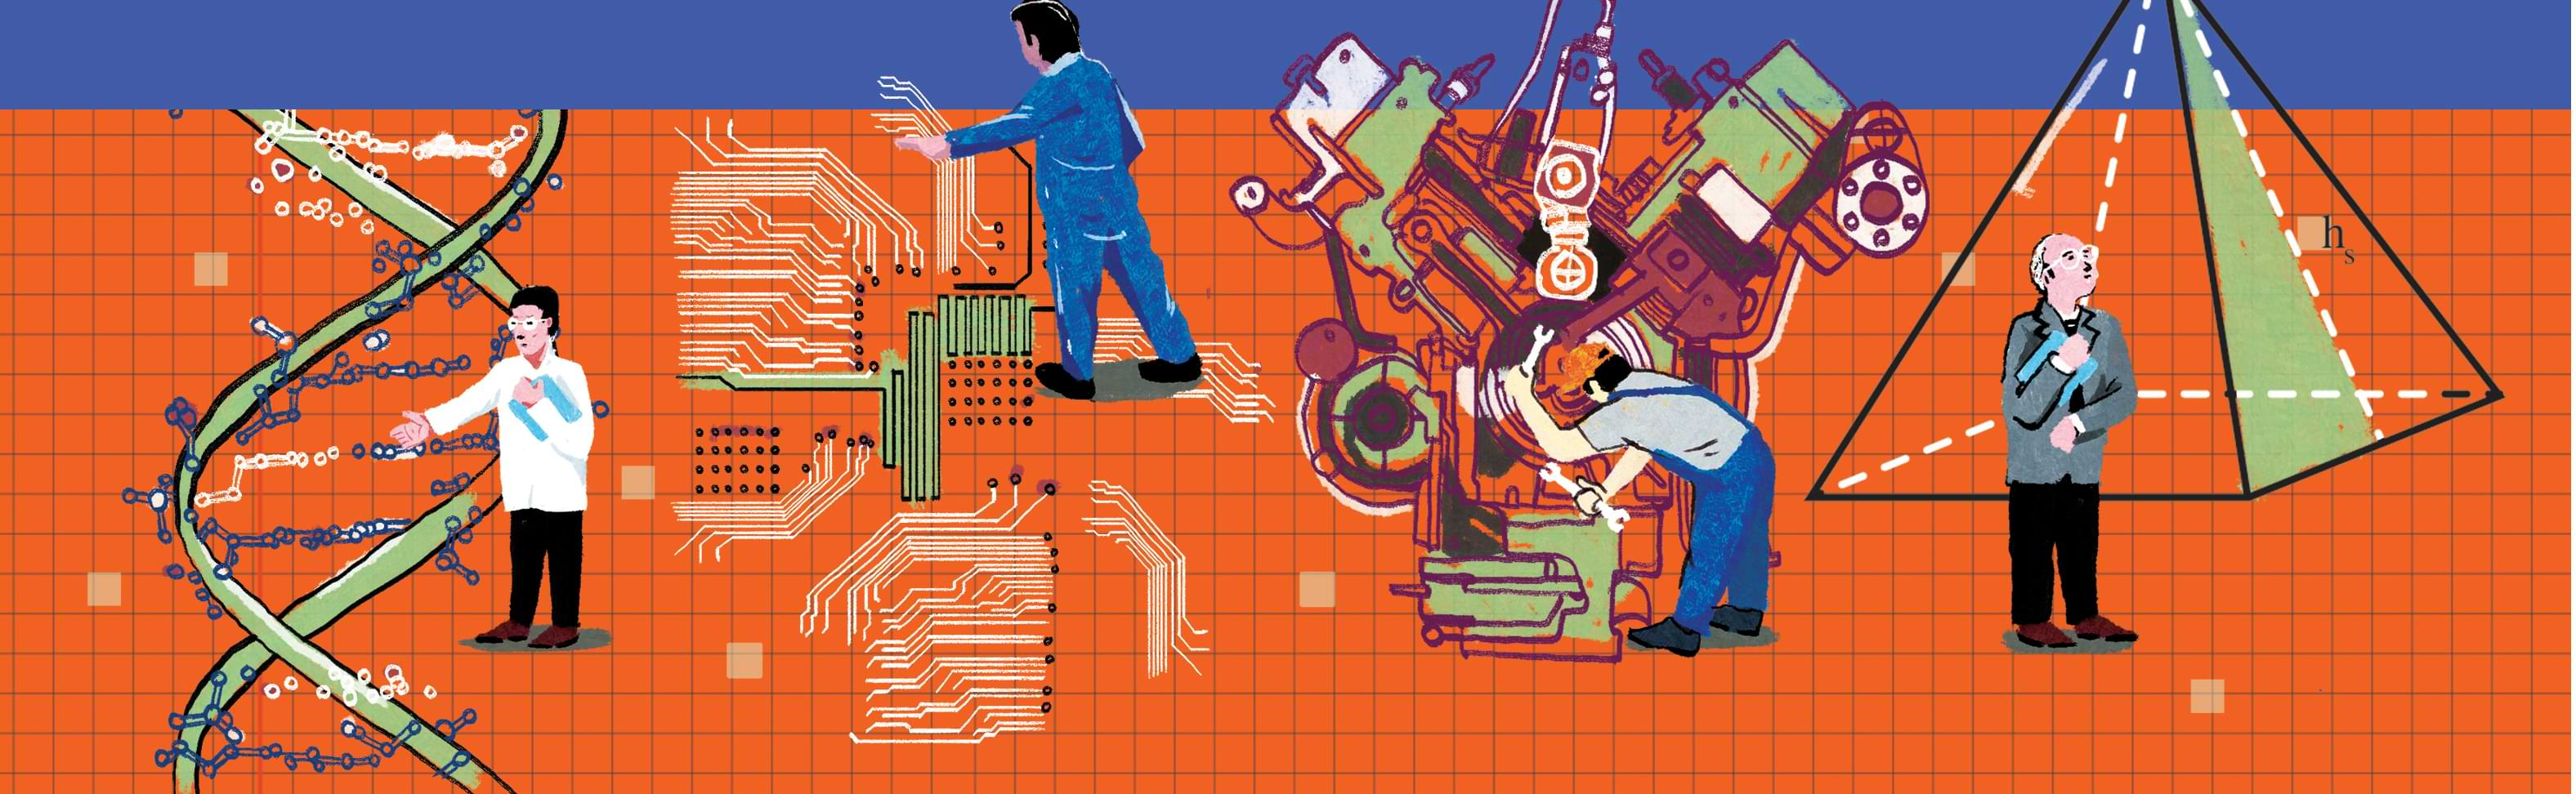
\includegraphics[width=19.3cm]{../bannertimhieu}}}
\AddToShipoutPicture*{\put(60,525){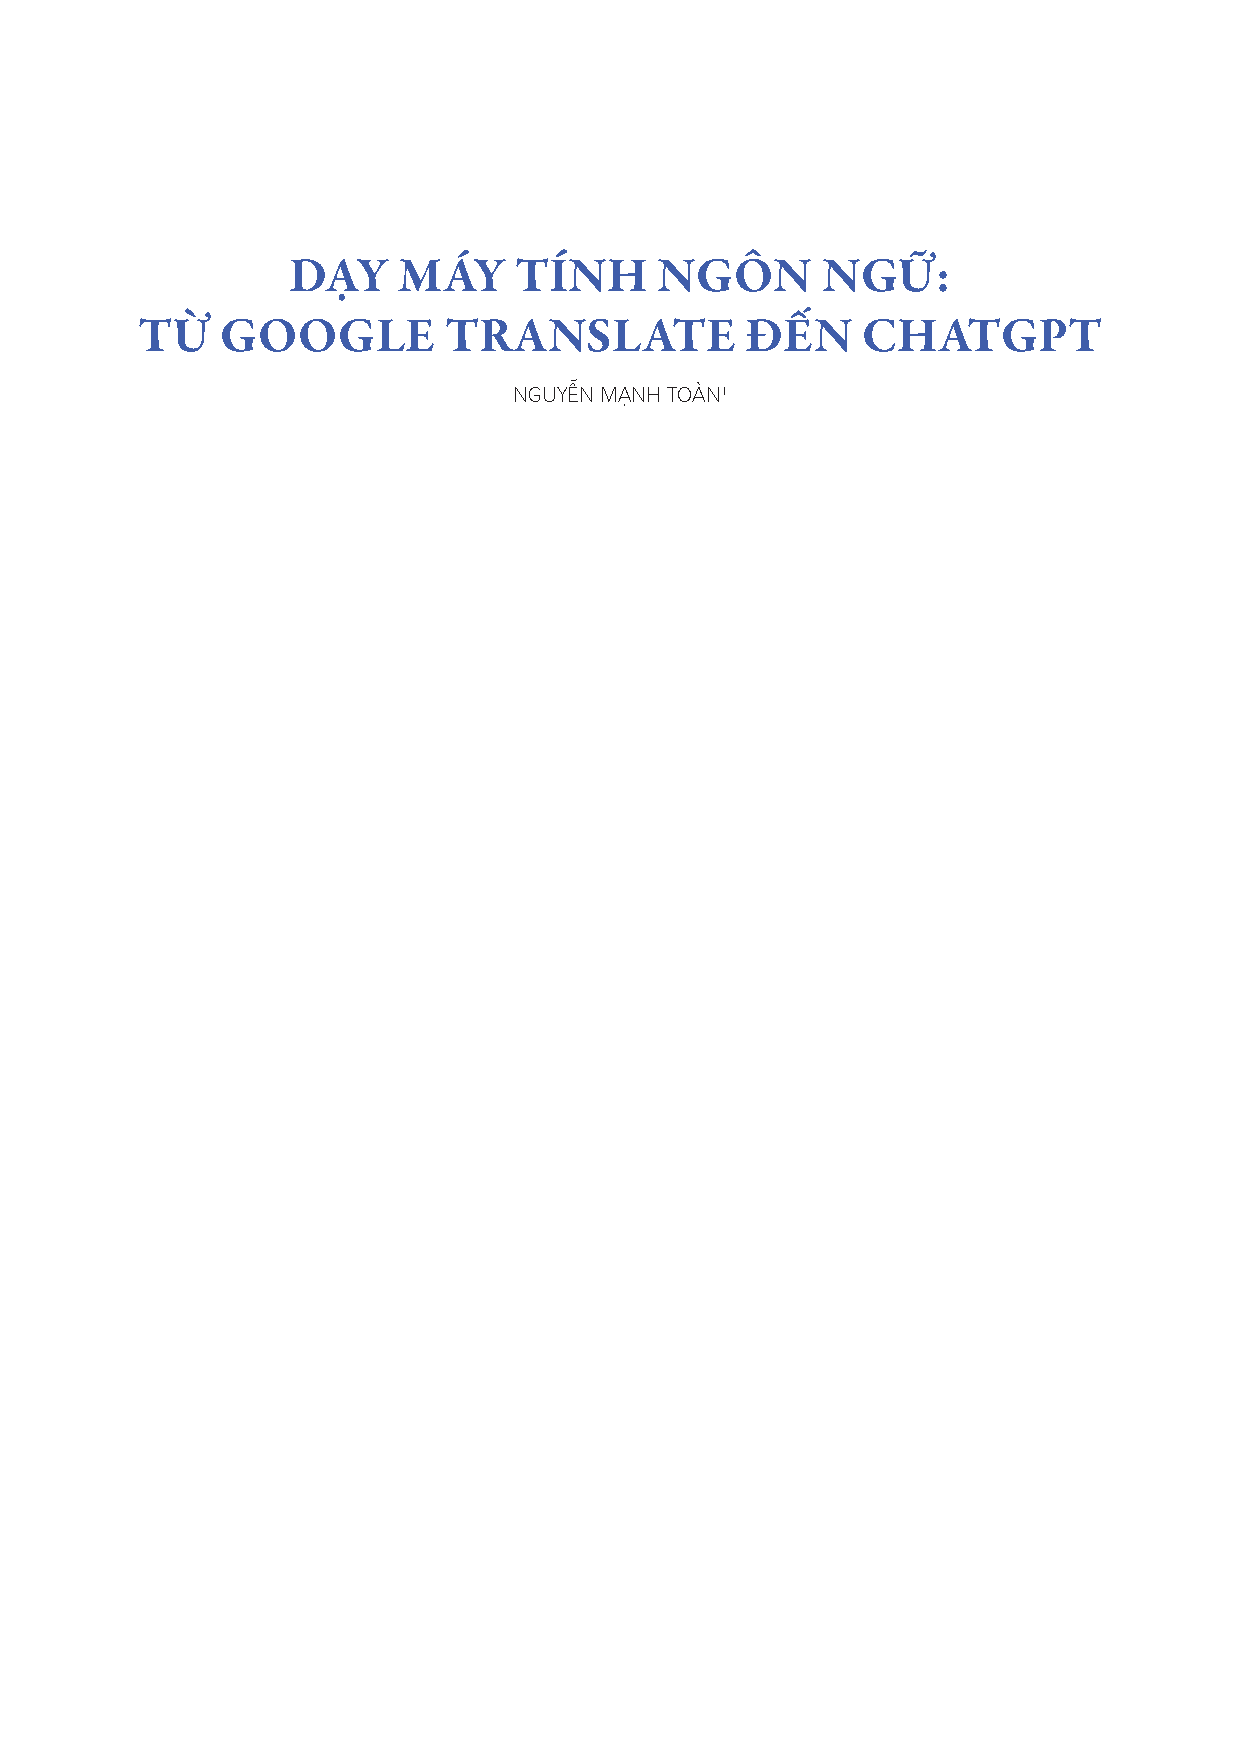
\includegraphics[scale=1]{../tieude.pdf}}}
\centering
\endgroup
\vspace*{180pt}

\begin{multicols}{2}
	\begin{figure}[H]
		\vspace*{5pt}
		\centering
		\captionsetup{labelformat= empty, justification=centering}
		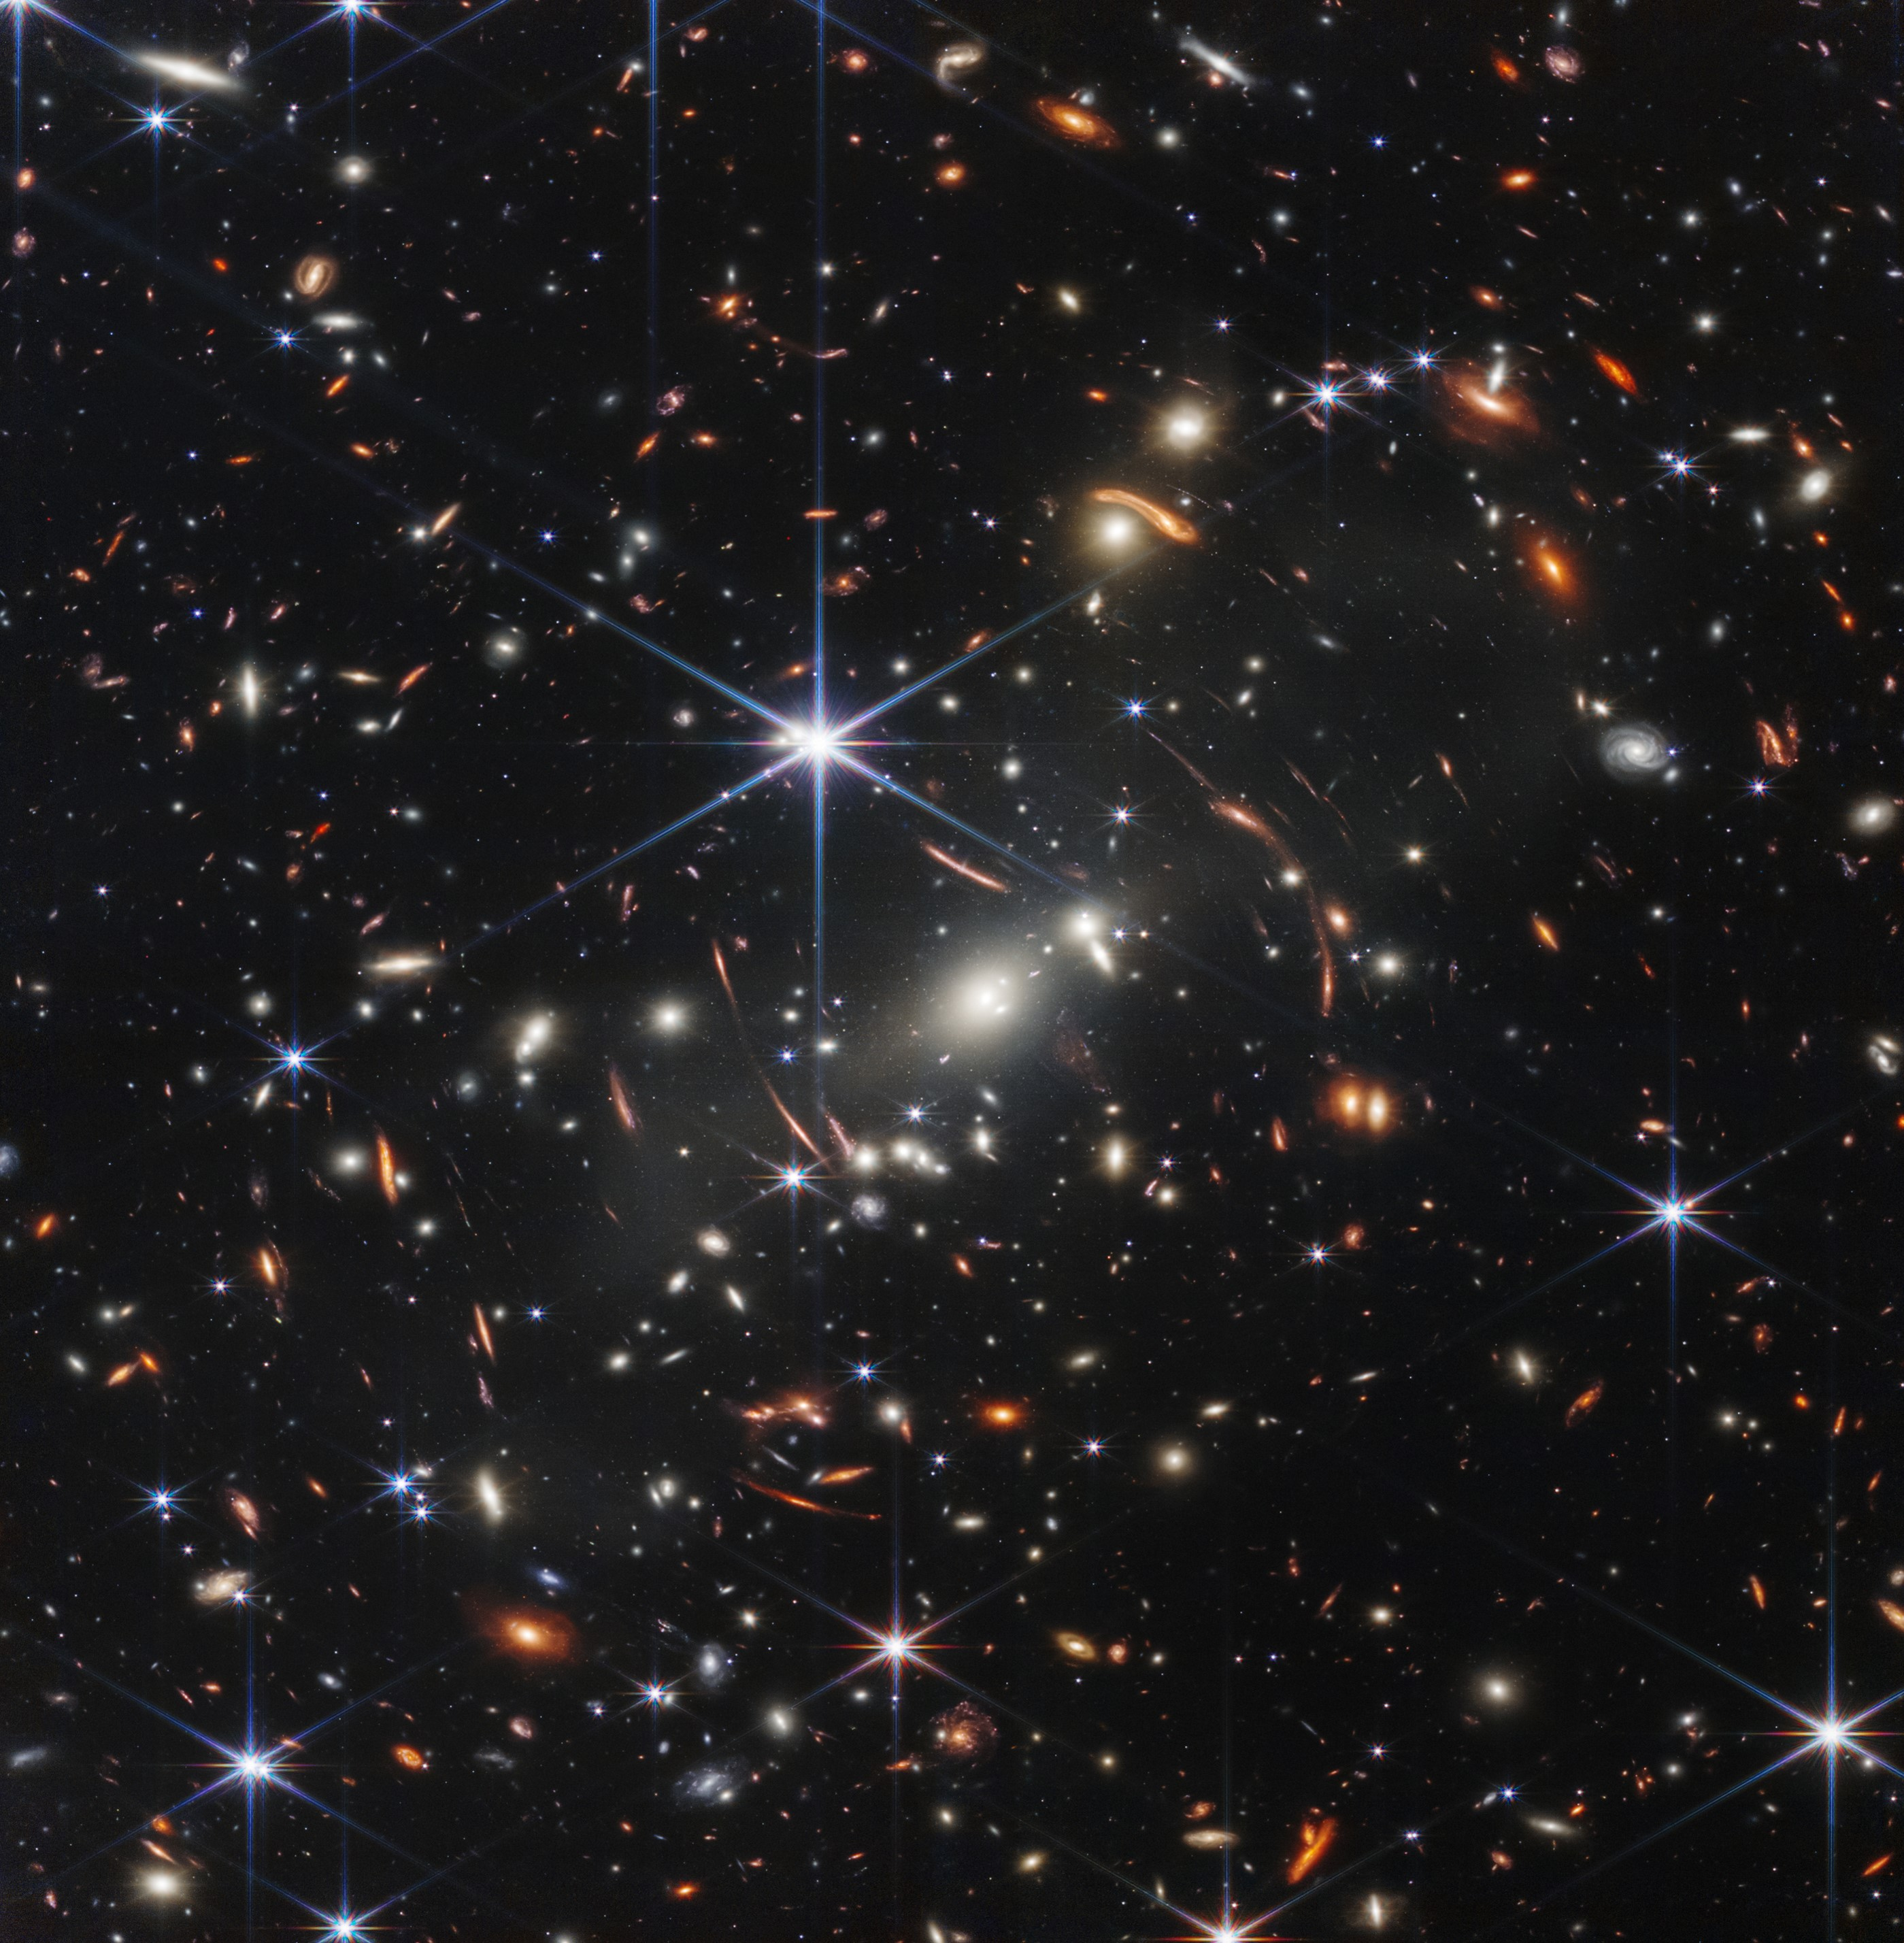
\includegraphics[width= 1\linewidth]{1}
		\caption{\small\textit{\color{timhieukhoahoc}Hình $1$. Ngay cả một điểm tương đương với một chấm nhỏ trên bầu trời trong mắt thường khi chụp bằng các kính thiên văn hiện đại cũng cho thấy rất nhiều các thiên hà và ngôi sao. Các vật thể này có vị trí thế nào trong bản đồ của vũ trụ vẫn luôn là một bài toán quan trọng của ngành thiên văn học.}}
		\vspace*{-10pt}
	\end{figure}
	Mỗi khi nhìn lên bầu trời với vô số các vì sao, bạn có từng đặt ra câu hỏi những ngôi sao này cách chúng ta bao xa? Đã từ lâu, cùng với việc quan sát những vì sao trên bầu trời, người ta cũng tìm nhiều cách khác nhau để đo khoảng cách từ chúng đến Trái Đất. Trong bài viết này, chúng ta hãy cùng tìm hiểu về phương pháp đo khoảng cách được nhà thiên văn học Henrietta Leavitt tìm ra vào đầu thế kỷ $20$ sử dụng biểu đồ log, cùng những ảnh hưởng sâu sắc của công thức này đến sự phát triển của thiên văn học hiện đại.
	
	$\pmb{1.}$ \textbf{\color{timhieukhoahoc}Leavitt và mối quan hệ chu kỳ -- độ sáng}
	\vskip 0.1cm
	Henrietta Swan Leavitt sinh năm $1868$ trong một gia đình trung lưu ở bang Massachusett, Mỹ. Bà được gia đình cho theo học đại học cho đến khi tốt nghiệp năm $24$ tuổi. Sau đó, Leavitt làm việc tình nguyện ở đài thiên văn Havard để có cơ hội học lên cao hơn.
	\vskip 0.1cm
	Giám đốc đài thiên văn Havard lúc đó là Edward Pickering, người đã điều hành đài thiên văn từ năm $1876$ khi mới $30$ tuổi. Những nhân viên dưới quyền Pickering thường là các phụ nữ đảm nhiệm các công việc lặp đi lặp lại xử lý dữ liệu từ các kính thiên văn cũng như tiến hành tính toán. Những người phụ nữ làm loại công việc này lúc đó được gọi là các ``computer" (trước khi từ này được dùng để chỉ máy tính điện tử). Tiền lương của họ cũng chỉ ngang với lương cơ bản: $25$ xu/giờ. Do lương thấp cùng sự đòi hỏi tính nhẫn nại và tỷ mỉ trong lao động, nam giới thường không làm các công việc này. Tất nhiên là Pickering cũng không hề có vấn đề gì khi nhận thêm một ``computer" miễn phí như Leavitt. 
	\begin{figure}[H]
		\vspace*{-5pt}
		\centering
		\captionsetup{labelformat= empty, justification=centering}
		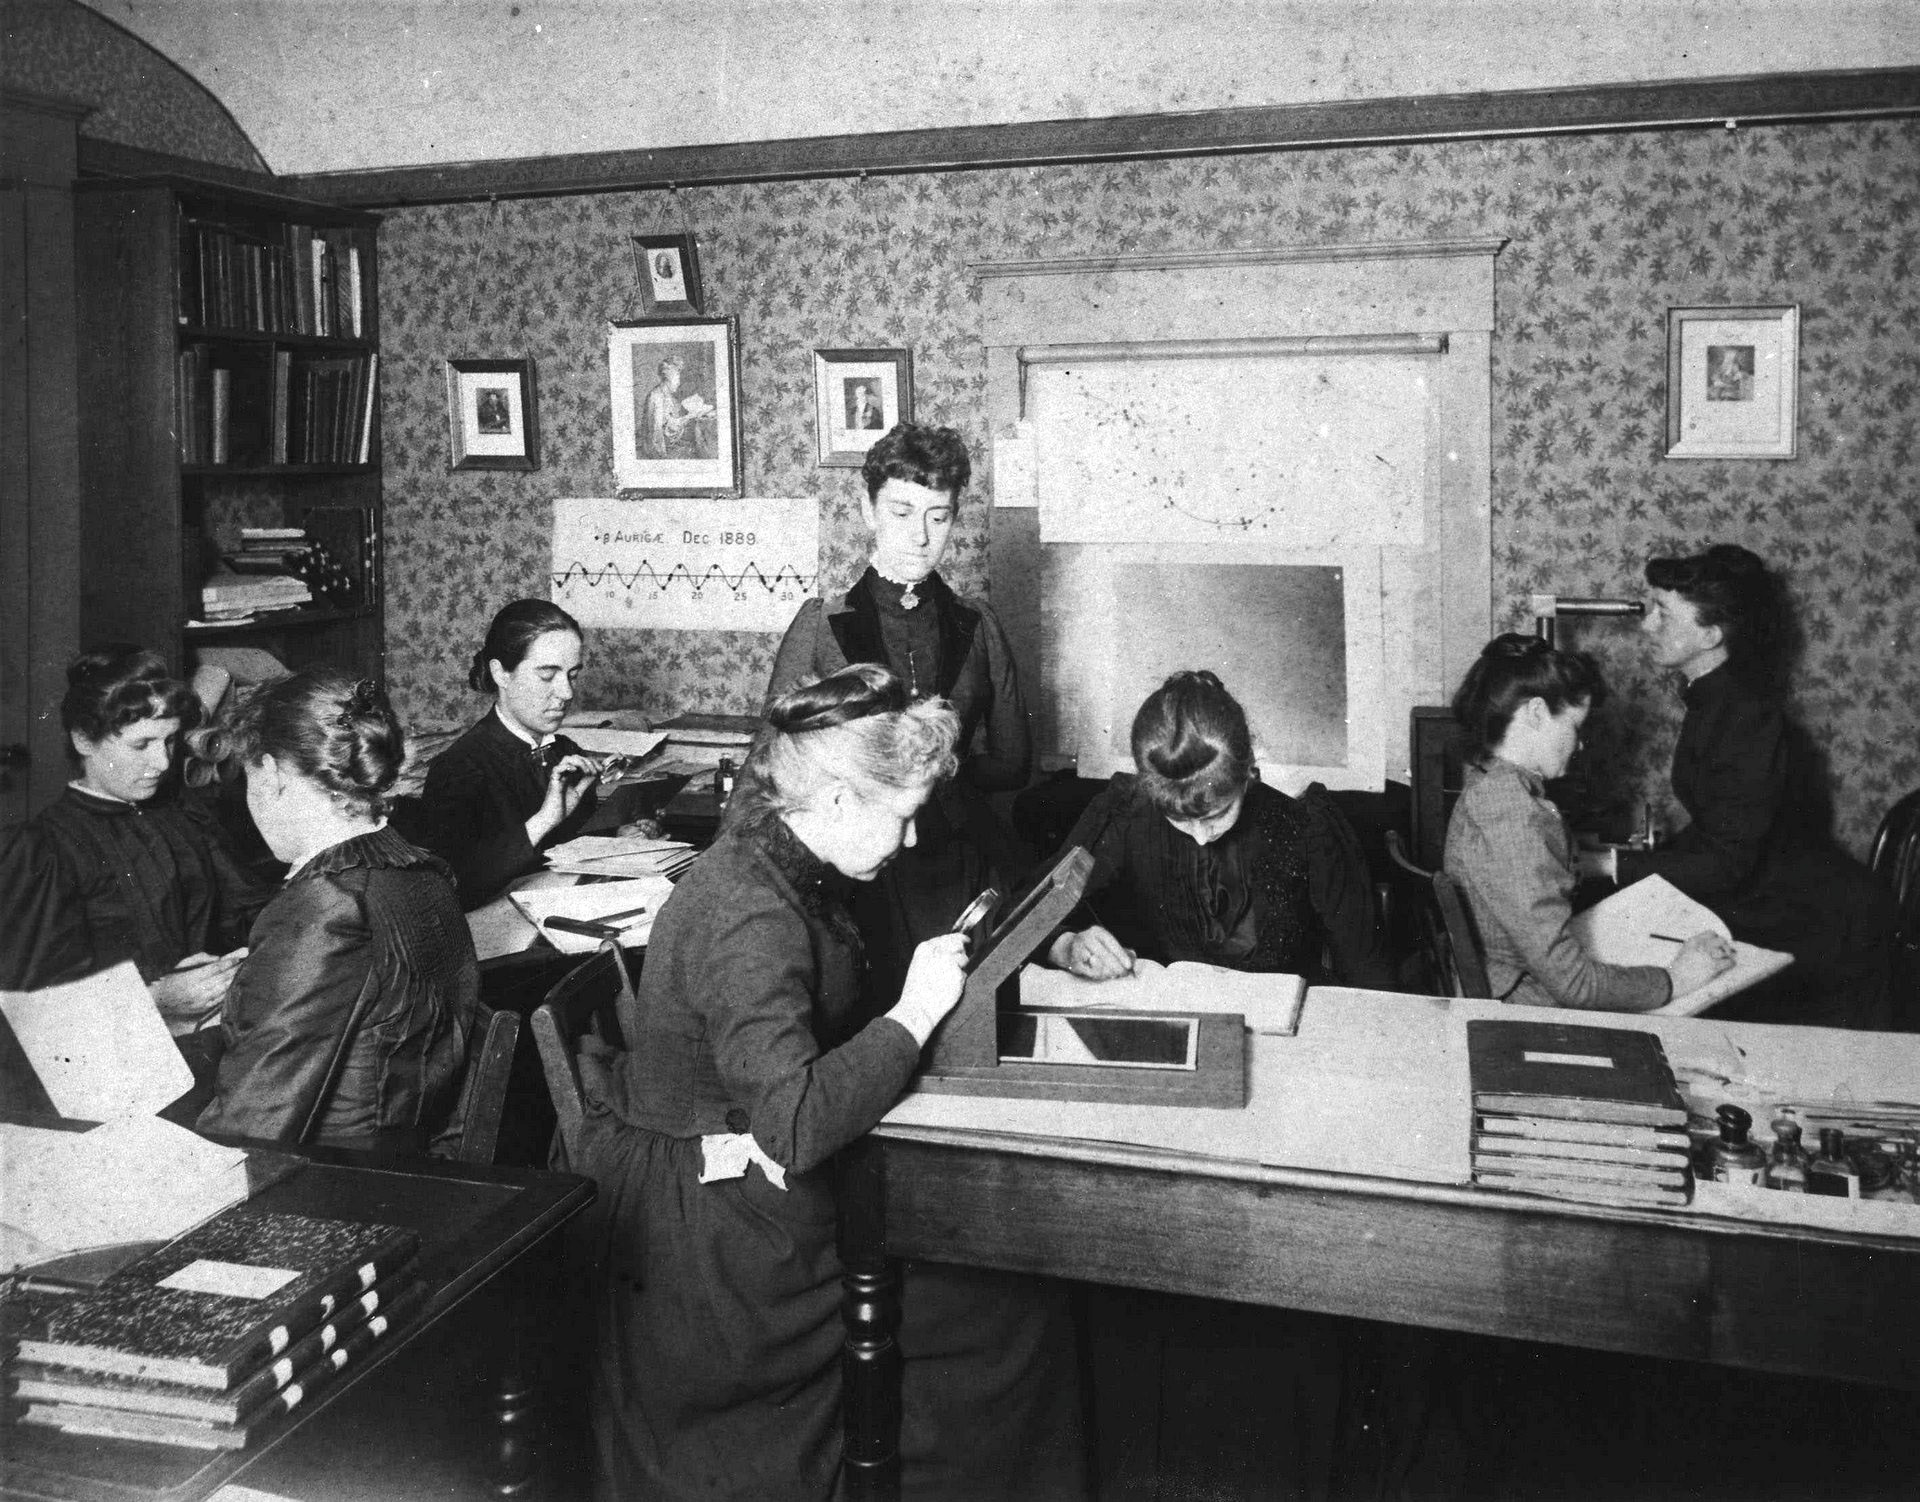
\includegraphics[width= 1\linewidth]{2}
		\caption{\small\textit{\color{timhieukhoahoc}Hình $2$. Những ``computer" ở Harvard dưới thời Pickering. Leavitt ngồi ở vị trí  thứ $3$ từ bên trái.}}
		\vspace*{-10pt}
	\end{figure}
	Dưới sự phân công của Pickering, Leavitt tiến hành xử lý những tấm phim ghi hình các ngôi sao được chụp qua kính viễn vọng. Trong cùng một thời gian phơi sáng, những ngôi sao sáng hơn sẽ để lại các đốm to hơn trên một tấm phim, tức là làm cho nhiều hạt trên phim bị tối đi hơn. Thông qua một kính lúp, Leavitt so sánh mỗi ngôi sao quan sát được với độ sáng của các ngôi sao đã biết và ghi lại các kết quả vào một cuốn sổ.
	\vskip 0.1cm
	Một công việc Leavitt thường xuyên phải làm là tìm kiếm các ngôi sao biến quang, chúng có độ sáng lên xuống theo chu kỳ, có thể kéo dài vài ngày, vài năm hoặc thậm chí vài tháng. Để xác định các ngôi sao này, người ta cần lấy hai tấm phim chụp cùng một vùng bầu trời ở hai thời điểm khác nhau, một tấm là phim dương bản còn một tấm là phim âm bản. Khi chồng khớp lên, nhau, những ngôi sao có độ sáng không đổi sẽ triệt tiêu, chỉ còn lại những ngôi sao mà độ sáng ở hai thời điểm là khác nhau. Sau khi các ngôi sao này được phát hiện, nhiều tấm phim hơn chụp cùng vị trí bầu trời ở các thời điểm khác sẽ được lấy ra đo đạc để xác định chu kỳ.
	\vskip 0.1cm
	Leavitt cần mẫn thực hiện công việc với các sao biến quang cho đến năm $1896$. Sau khi đi sang châu Âu hai năm, bà trở lại Boston, và mang theo bản thảo nghiên cứu của mình về Beloit, bang Wisconsin. Trong khi cha của Leavitt làm mục sư ở đây thì bà trở thành trợ giảng nghệ thuật tại Beloit College. Năm $1902$, Leavitt liên lạc lại với Pickering và muốn tiếp tục công việc liên quan đến thiên văn học.
	\begin{figure}[H]
		\vspace*{-5pt}
		\centering
		\captionsetup{labelformat= empty, justification=centering}
		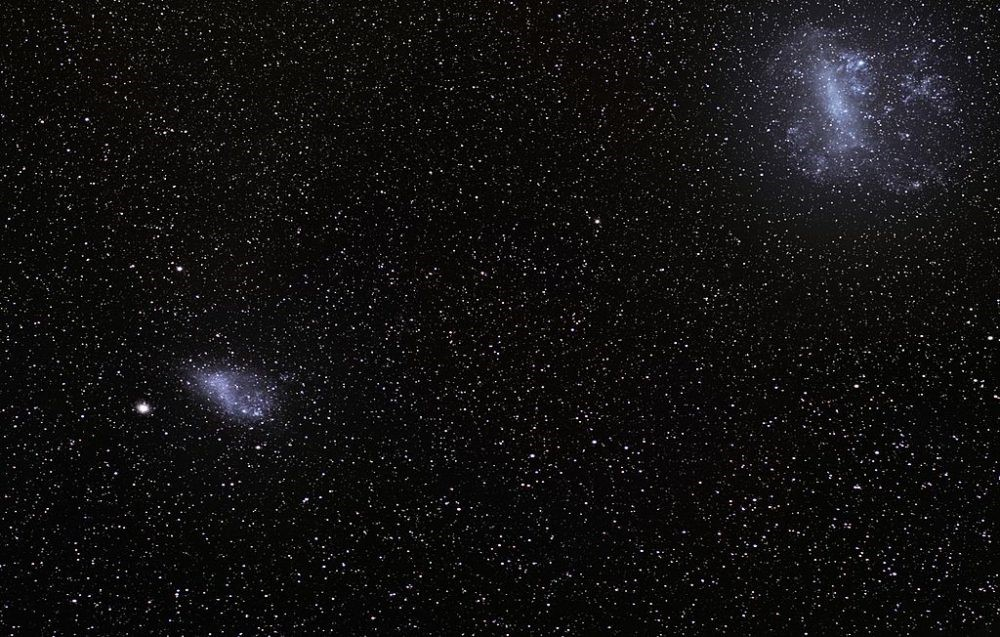
\includegraphics[width= 1\linewidth]{3}
		\caption{\small\textit{\color{timhieukhoahoc}Hình $3$. Các đám mây Magellan quan sát từ Trái Đất. Ngày nay người ta đã biết chúng là hai thiên hà vệ tinh của dải Ngân hà của chúng ta.}}
		\vspace*{-10pt}
	\end{figure}
	Vào mùa xuân năm $1904$, Leavitt bắt đầu phát hiện các ngôi sao biến quang nằm trong đám mây Magellan nhỏ. Tiếp theo đó, nhiều ngôi sao biến quang khác cũng được bà phát hiện. Đến năm $1908$, riêng một mình Leavitt đã phát hiện được tổng cộng $1777$ sao biến quang ở hai đám mây Magellan. Không chỉ có thế, bà còn đưa ra một nhận định rất quan trọng từ dữ liệu của $16$ ngôi sao trong số đó: các ngôi sao sáng hơn sẽ có chu kỳ dài hơn.
	\begin{figure}[H]
		\vspace*{-5pt}
		\centering
		\captionsetup{labelformat= empty, justification=centering}
		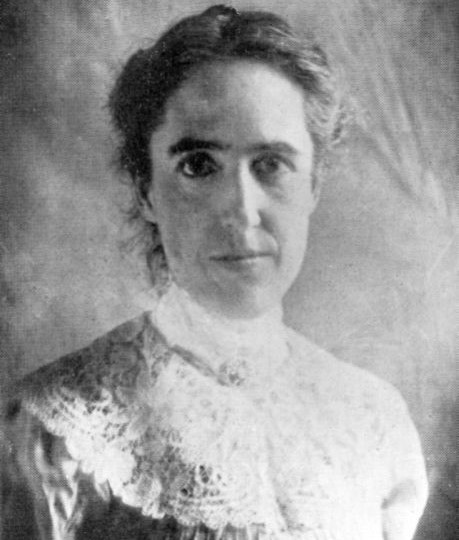
\includegraphics[width= 0.7\linewidth]{4}
		\caption{\small\textit{\color{timhieukhoahoc}Henrietta Swan Leavitt $(1868 - 1921)$.}}
		\vspace*{-5pt}
	\end{figure}
	Để tìm ra quy luật chi tiết hơn, cỡ mẫu $16$ ngôi sao là không đủ nhưng công việc lại bị gián đoạn do Leavitt gặp nhiều vấn đề về sức khỏe cũng như việc cha của bà qua đời năm $1910$. Mãi một thời gian sau, Leavitt mới có thể tập trung trở lại cho việc phân tích số liệu về các sao biến quang. 
	\vskip 0.1cm
	Năm $1912$, các kết quả của Leavitt được công bố kèm trong bài báo của Pickering. Biểu đồ dữ liệu của $25$ ngôi sao cho thấy độ sáng trung bình quan sát được của chúng tỷ lệ thuận với \textit{log} của chu kỳ. Các ngôi sao càng sáng sẽ có chu kỳ càng dài. Đồng thời, các ngôi sao này ở cùng trong một đám mây Magellan nên khoảng cách từ chúng đến Trái Đất sẽ xấp xỉ như nhau. Điều đó mở ra khả năng ta có thể xác định được độ sáng thực của một ngôi sao chỉ với chu kỳ của nó rồi so sánh với độ sáng quan sát được tại Trái Đất để ước lượng khoảng cách (độ sáng quan sát được của một ngôi sao tại các điểm khác nhau trong vũ trụ sẽ tỷ lệ nghịch với bình phương khoảng cách). 
	\begin{figure}[H]
		\vspace*{-5pt}
		\centering
		\captionsetup{labelformat= empty, justification=centering}
		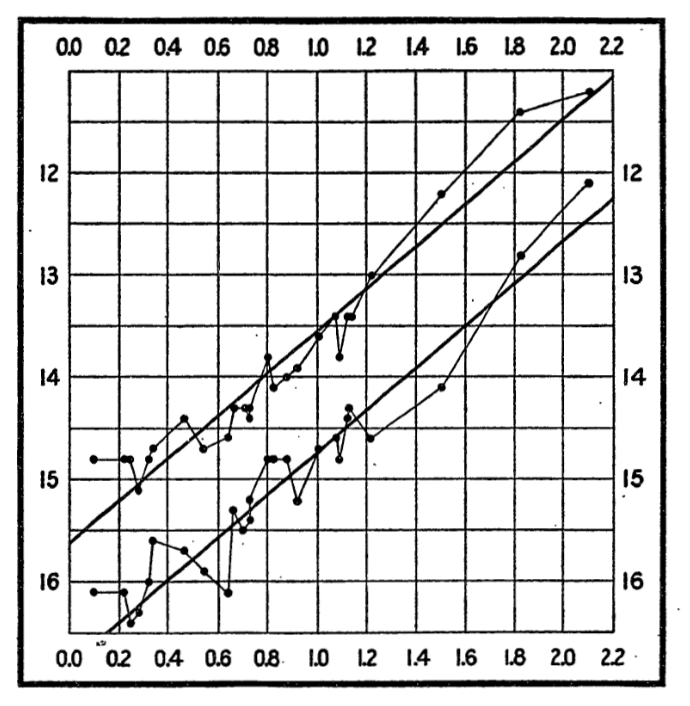
\includegraphics[width= 1\linewidth]{5}
		\caption{\small\textit{\color{timhieukhoahoc}Hình $4$. Biểu đồ của Leavitt cho thấy độ sáng quan sát được của các sao biến quang trong đám mây Magellan (trục thẳng đứng) tỷ lệ với log của chu kỳ của chúng.}}
		\vspace*{-10pt}
	\end{figure}
	Không phải ngôi sao nào cũng có độ sáng thay đổi theo chu kỳ. Những ngôi sao tuân theo quy luật mà Leavitt nêu ra còn được gọi là các sao Cepheid. Chúng được phát hiện lần đầu năm $1784$ trong chòm sao Cepheus bởi nhà thiên văn học nghiệp dư John Goodricke. Vấn đề còn lại để công thức của Leavitt có thể sử dụng được chính là việc tính các hệ số của nó từ các ngôi sao mà ta có thể xác định được khoảng cách theo năm ánh sáng.
	\vskip 0.1cm
	Trong hình học, khi biết độ lớn của một cạnh trong tam giác và độ lớn của hai góc kề cạnh này, ta có thể tính được độ dài của hai cạnh còn lại. Đây chính là cơ sở của phương pháp thị sai trong thiên văn học. Theo đó, người ta quan sát cùng một vật thể trên bầu trời tại hai địa điểm khác nhau vào cùng một thời điểm và đo góc quan sát so với mặt đất tại hai địa điểm này. Nếu biết khoảng cách giữa hai địa điểm, ta có thể tính được khoảng cách từ mỗi điểm đến vật thể.
	\vskip 0.1cm
	Vào thế kỷ thứ hai trước Công nguyên, nhà toán học Hipparchus đã dùng phương pháp thị sai để tính khoảng cách giữa Trái Đất và Mặt Trăng. Vào cùng một thời điểm, nhật thực toàn phần xảy ra ở thành phố Hellespont, trong khi ở Alexandria, Mặt Trăng chỉ che đi $4/5$ đường kính Mặt Trời. Từ vĩ độ của hai thành phố, Hipparchus tính ra rằng khoảng cách từ Trái Đất đến Mặt Trăng gấp khoảng $30$ lần đường kính Trái Đất, rất gần với kết quả đo được bằng tín hiệu radar ngày nay. Vào thế kỷ $18$, người ta cũng đo khoảng cách đến sao Kim một cách tương tự khi nó đi ngang qua trước Mặt Trời.
	\begin{figure}[H]
		\vspace*{-5pt}
		\centering
		\captionsetup{labelformat= empty, justification=centering}
		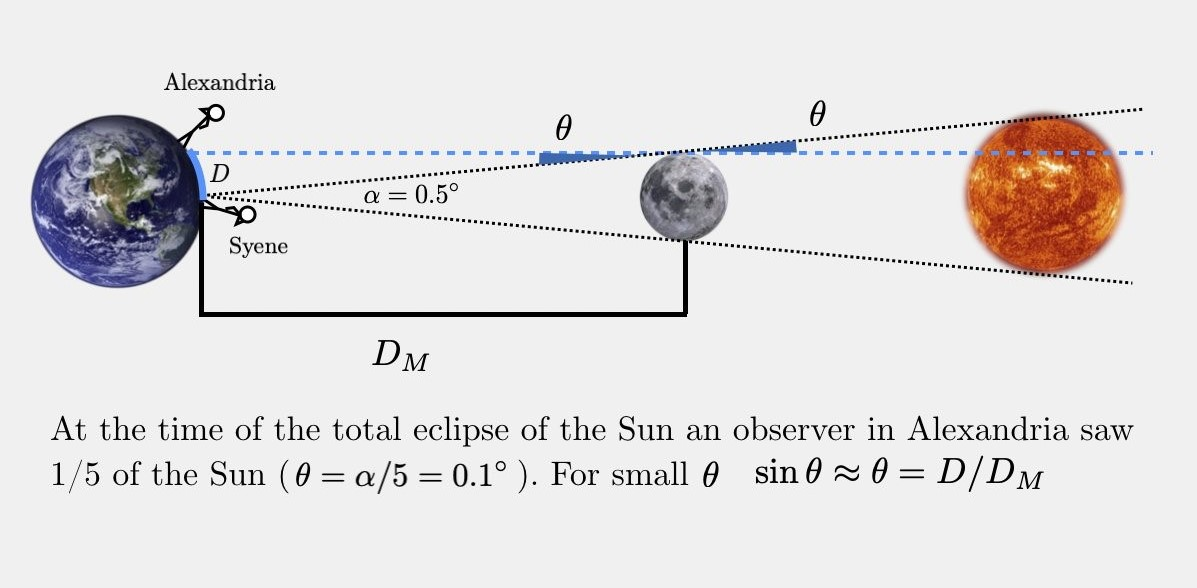
\includegraphics[width= 1\linewidth]{6}
		\caption{\small\textit{\color{timhieukhoahoc}Hình $5$. Phương pháp thị sai mà Hipparchus đã dùng để đo khoảng cách tới Mặt Trăng.}}
		\vspace*{-5pt}
	\end{figure}
	Với những vật thể ở khoảng cách xa hơn, phương pháp thị sai dạng như trên không khả thi do bị giới hạn bởi độ chính xác của phép đo góc. Để giải quyết việc này, người ta tiến hành đo góc từ cùng một vị trí trên Trái Đất tới cùng một vật thể trên bầu trời ở hai thời điểm cách nhau $6$ tháng, khi mà Trái Đất ở vào các điểm đầu bán trục lớn của quỹ đạo ellipse quay quanh Mặt Trời. Khoảng cách này đủ lớn để độ chênh lệch góc giữa hai vị trí có thể đo được. Đến thế kỷ $19$, người ta đã đo được khoảng cách từ Trái Đất đến nhiều ngôi sao khác nhau bằng cách này.
	\begin{figure}[H]
		\vspace*{-5pt}
		\centering
		\captionsetup{labelformat= empty, justification=centering}
		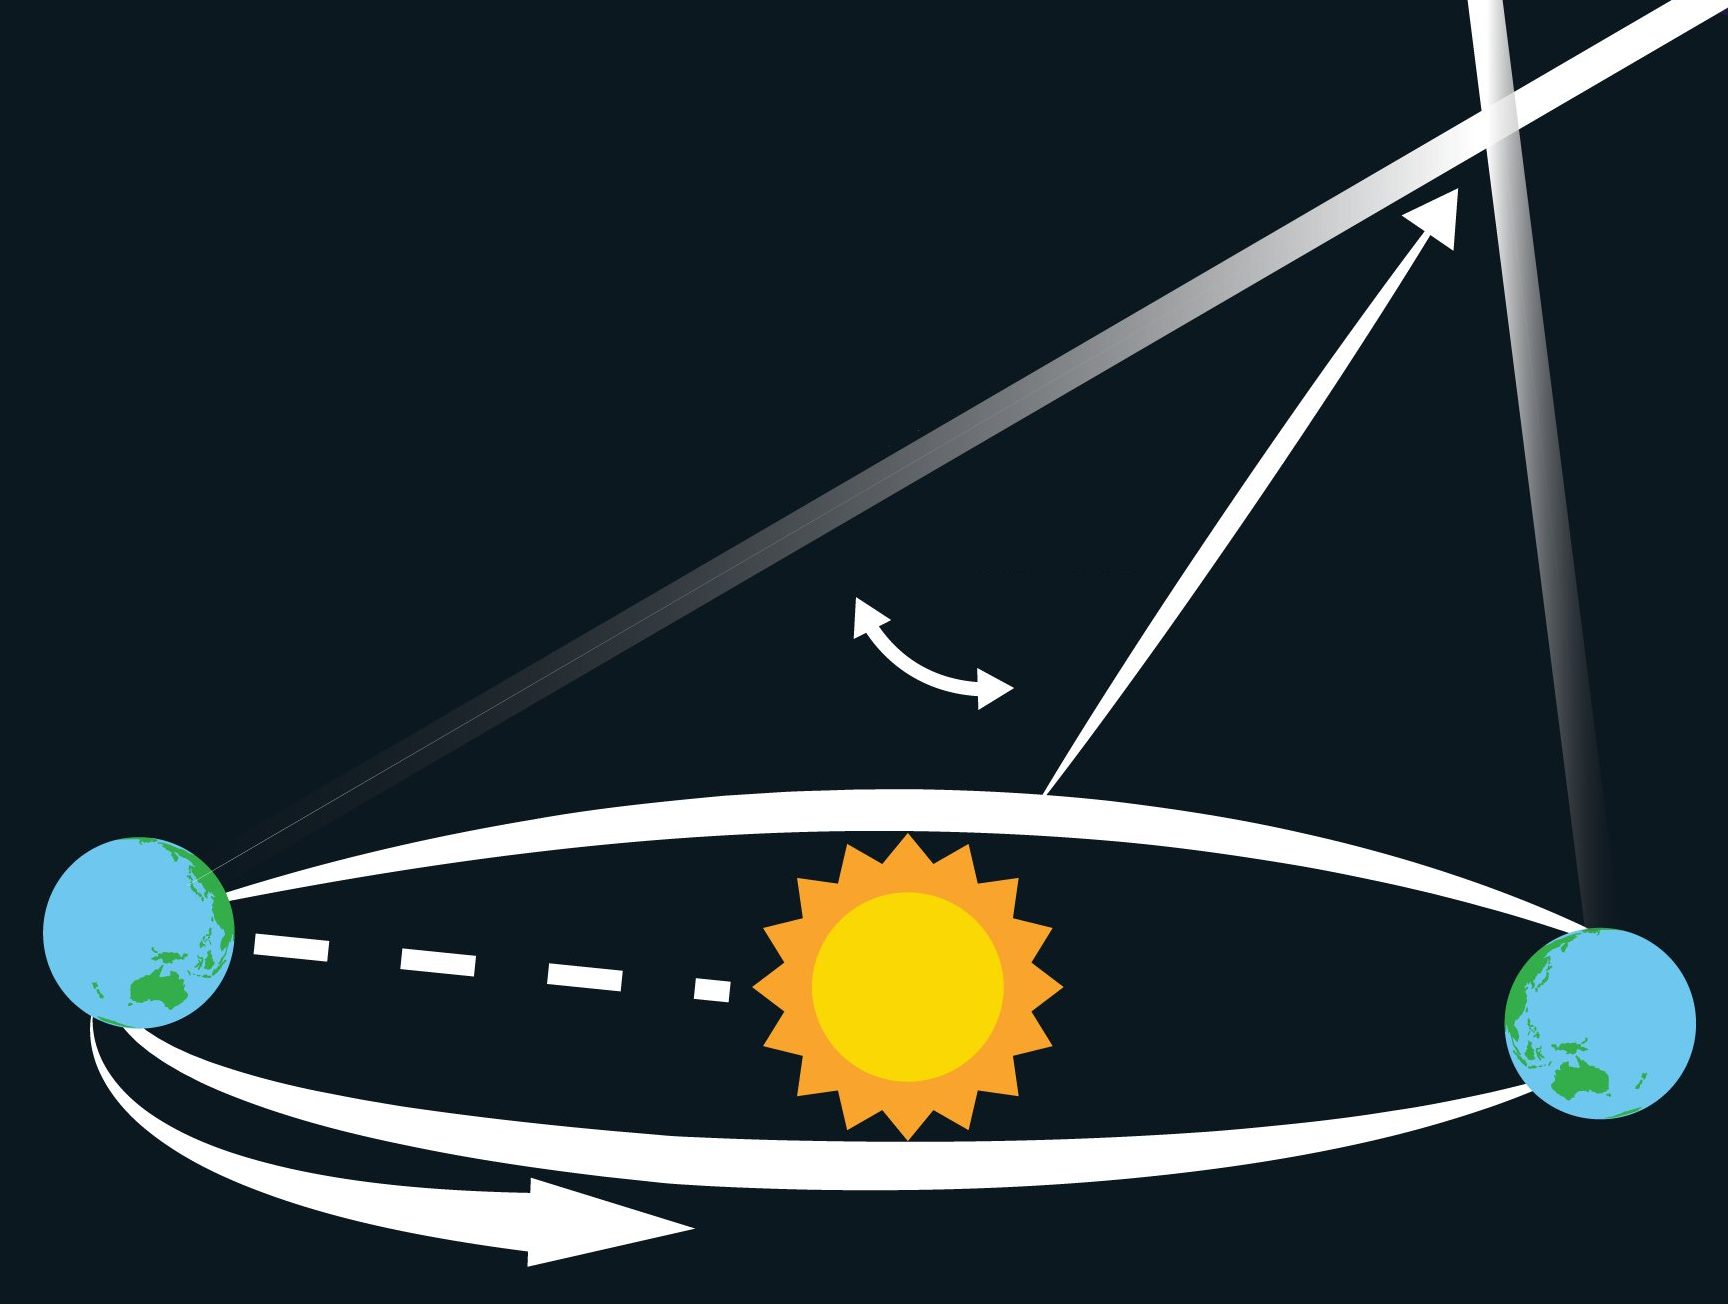
\includegraphics[width= 1\linewidth]{7}
		\caption{\small\textit{\color{timhieukhoahoc}Hình $6$. Phương pháp thị sai sử dụng hai điểm trên quỹ đạo của Trái Đất quanh Mặt Trời làm điểm quan sát.}}
		\vspace*{-10pt}
	\end{figure}
	Tuy nhiên, phần lớn các ngôi sao trên bầu trời ở quá xa để có thể đo khoảng cách bằng phương pháp trên, bao gồm các sao Cepheid mà chúng ta đã nói. Phải đến năm $1913$, nhà thiên văn học Ejnar Hertzsprung mới đo được khoảng cách đến một số ngôi sao Cepheid trong dải Ngân Hà của chúng ta. Ông sử dụng một hiện tượng đã được nhà thiên văn học William Herschel phát hiện từ thế kỷ $18$: Mặt Trời cũng chuyển động trong vũ trụ. Herschel nhận thấy điều này nhờ quan sát hai chòm sao Hercules và Columba. Khi quan sát từ Trái Đất, các ngôi sao của Hercules có xu hướng tán ra theo thời gian còn các ngôi sao của Columa lại cụm dần lại. Vận tốc chuyển động của Mặt Trời được ước tính vào khoảng $20$ km/s. Khi tiến hành phương pháp đo thị sai ở hai thời điểm cách nhau nhiều năm, hệ Mặt Trời đã di chuyển đủ nhiều để ta có thể xác định một số khoảng cách đến các vật thể vũ trụ xa hơn. Các tính toán của Hertzsprung đã cung cấp các hệ số cho quan hệ mà Leavitt đã chỉ ra và đến lúc này, người ta đã có một công thức để tính khoảng cách đến các ngôi sao Cepheid chỉ dựa vào chu kỳ của chúng.
	\vskip 0.1cm
	$\pmb{2.}$ \textbf{\color{timhieukhoahoc}Harlow Shapley và kích thước của dải Ngân hà}
	\vskip 0.1cm
	Vào thế kỷ $18$, trong ngành thiên văn học xảy ra cuộc tranh cãi về bản chất của các tinh vân (\textit{nebula} trong thuật ngữ ngành thiên văn). Nhà thiên văn học William Herschel và nhà triết học Immanuel Kant cho rằng các tinh vân mà ta quan sát được thực chất là các thiên hà ở xa và gồm nhiều hệ Mặt Trời, tương tự như dải Ngân hà của chúng ta. Đây còn được gọi là thuyết ``các vũ trụ dạng hòn đảo". Trong khi đó, nhà toán học Laplace lại cho rằng các tinh vân thực chất là các đám mây khí có dạng xoắn ốc xung quanh một ngôi sao nằm trong dải Ngân hà, chứ không phải hệ các ngôi sao. Cuộc tranh cãi vẫn còn tiếp diễn đến đầu thế kỷ $20$.
	\vskip 0.1cm
	Với các đo đạc dựa trên hiệu ứng Doppler, năm $1914$, người ta đã phát hiện được rằng các tinh vân chuyển động với vận tốc rất nhanh (có thể lên đến $1000$ km/s). Cùng với một số số liệu khác về các nova (vụ nổ tân tinh) quan sát được, nhiều người đã cho rằng các tinh vân là các thiên hà riêng biệt. Trong số đó, một nhà thiên văn học trẻ là Harlow Shapley bắt đầu chú ý đến phát hiện mới của Leavitt về quy luật của các sao Cepheid. Shapley bắt đầu nảy ra ý tưởng dùng phương pháp tính khoảng cách sử dụng các Cepheid để xác định kích thước và hình dạng của dải Ngân hà mà hệ Mặt Trời của chúng ta đang tồn tại trong đó.
	\vskip 0.1cm
	Năm $1914$, Shapley bắt đầu tiến hành nghiên cứu các cụm sao hình cầu (globular cluster) nằm rải rác trong dải Ngân hà cùng các ngôi sao biến quang trong chúng. Kết quả Shapley thu được cho kích thước giữa hai đầu giải ngân hà là $300000$ năm ánh sáng, lớn hơn rất nhiều so với con số $25000$ được chấp nhận lúc đó (con số hiện nay là $100 000$ năm anh sáng với các mô hình và số liệu chính xác hơn nhiều thời của Shapley). Đồng thời, Shapley cũng phát hiện Mặt Trời không nằm ở trung tâm của dải Ngân hà như mọi người lúc đó vẫn tưởng tượng.
	\begin{figure}[H]
		\vspace*{-5pt}
		\centering
		\captionsetup{labelformat= empty, justification=centering}
		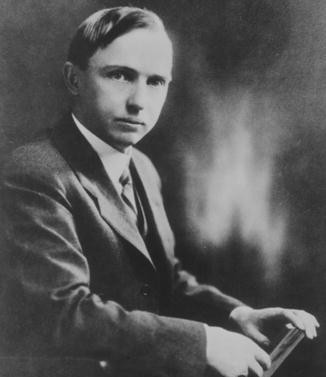
\includegraphics[width= 1\linewidth]{8}
		\caption{\small\textit{\color{timhieukhoahoc}Harlow Shapley $(1885 - 1972)$.}}
		\vspace*{-10pt}
	\end{figure}
	Giả sử rằng bản thân dải Ngân hà đã lớn như vậy thì nếu như các tinh vân là những thiên hà ở bên ngoài thì khoảng cách từ chúng đến ta còn vĩ đại hơn nhiều, đến hàng triệu năm ánh sáng hoặc hơn nữa. Với những hiểu biết về vũ trụ lúc đó, những khoảng cách lớn như vậy có vẻ là không chấp nhận được, ngay cả với Shapley. Đồng thời, Shapley cũng dựa trên nhận xét từ quan sát của nhà thiên văn học van Maanen rằng các tinh vân có chuyển động quay quan sát được. Các lý do trên làm cho Shapley chuyển sang nghĩ rằng các tinh vân chỉ là các đám mây khí như Laplace đã nói chứ không phải là các thiên hà riêng biệt.
	\vskip 0.1cm
	Năm $1920$, Shapley tham gia cuộc tranh luận trước công chúng với Herber Curtis, một nhà thiên văn học nổi tiếng đương thời. Curtis đại diện cho các quan điểm truyền thống lúc đó. Đây còn được gọi là ``cuộc tranh luận vĩ đại" (the Great Debate) đầu tiên của ngành thiên văn học. Cả hai người tham gia đều nghĩ rằng mình đã chiến thắng sau khi cuộc tranh luận kết thúc. Thực tế thì cả hai đều chỉ có một phần sự thật. Shapley đã đúng khi nói rằng rằng kích thước dải Ngân hà lớn hơn nhiều so với con số $25 000$ năm ánh sáng, cũng như việc hệ Mặt Trời không phải là trung tâm của vũ trụ. Curtis tuy không chấp nhận phương pháp đo sử dụng Cepheid nhưng cũng đưa ra một số nhận định đúng bao gồm: phổ bức xạ của các tinh vân tương tự như những cụm sao trong dải Ngân hà nên các tinh vân này là các thiên hà riêng biệt; và số liệu về chuyển động quay của các tinh vân mà van Maanen quan sát được có thể không đáng tin cậy (và thực sự là như vậy, tốc độ quay rất chậm của các tinh vân không phải là một đại lượng một con người có thể tiến hành quan sát trong vòng đời của mình). Đồng thời, trong khi Shapley lập luận rằng độ sáng của các nova quan sát được từ các tinh vân là quá cao so với giả thuyết rằng chúng là các thiên hà ở rất xa thì Curtis đã đúng khi nói rằng có thể có hai mức độ sáng của các nova chứ không phải một. Phải đến vài năm sau cuộc tranh luận của Shapley và Curtis thì những bằng chứng quyết định mới được hé lộ bởi một nhà thiên văn học khác: Edwin Hubble.
	\vskip 0.1cm
	$\pmb{3.}$ \textbf{\color{timhieukhoahoc}Hubble và sự dãn nở của vũ trụ}
	\vskip 0.1cm
	Hubble là con trai của một luật sư tại bang Missourim, Hoa Kỳ. Ông theo học luật ở Đại học Chicago và sau đó là đại học Oxford. Sau khi đi dạy trung học một thời gian, ông quay lại Chicago và học tiếp thành tiến sĩ ngành thiên văn học. Trong chiến tranh thế giới thứ I, Hubble là sĩ quan trong quân đội Mỹ ở châu Âu. Khi trở về, ông làm việc tại đài thiên văn núi Wilson, dưới quyền của Shapley.
	\begin{figure}[H]
		\vspace*{5pt}
		\centering
		\captionsetup{labelformat= empty, justification=centering}
		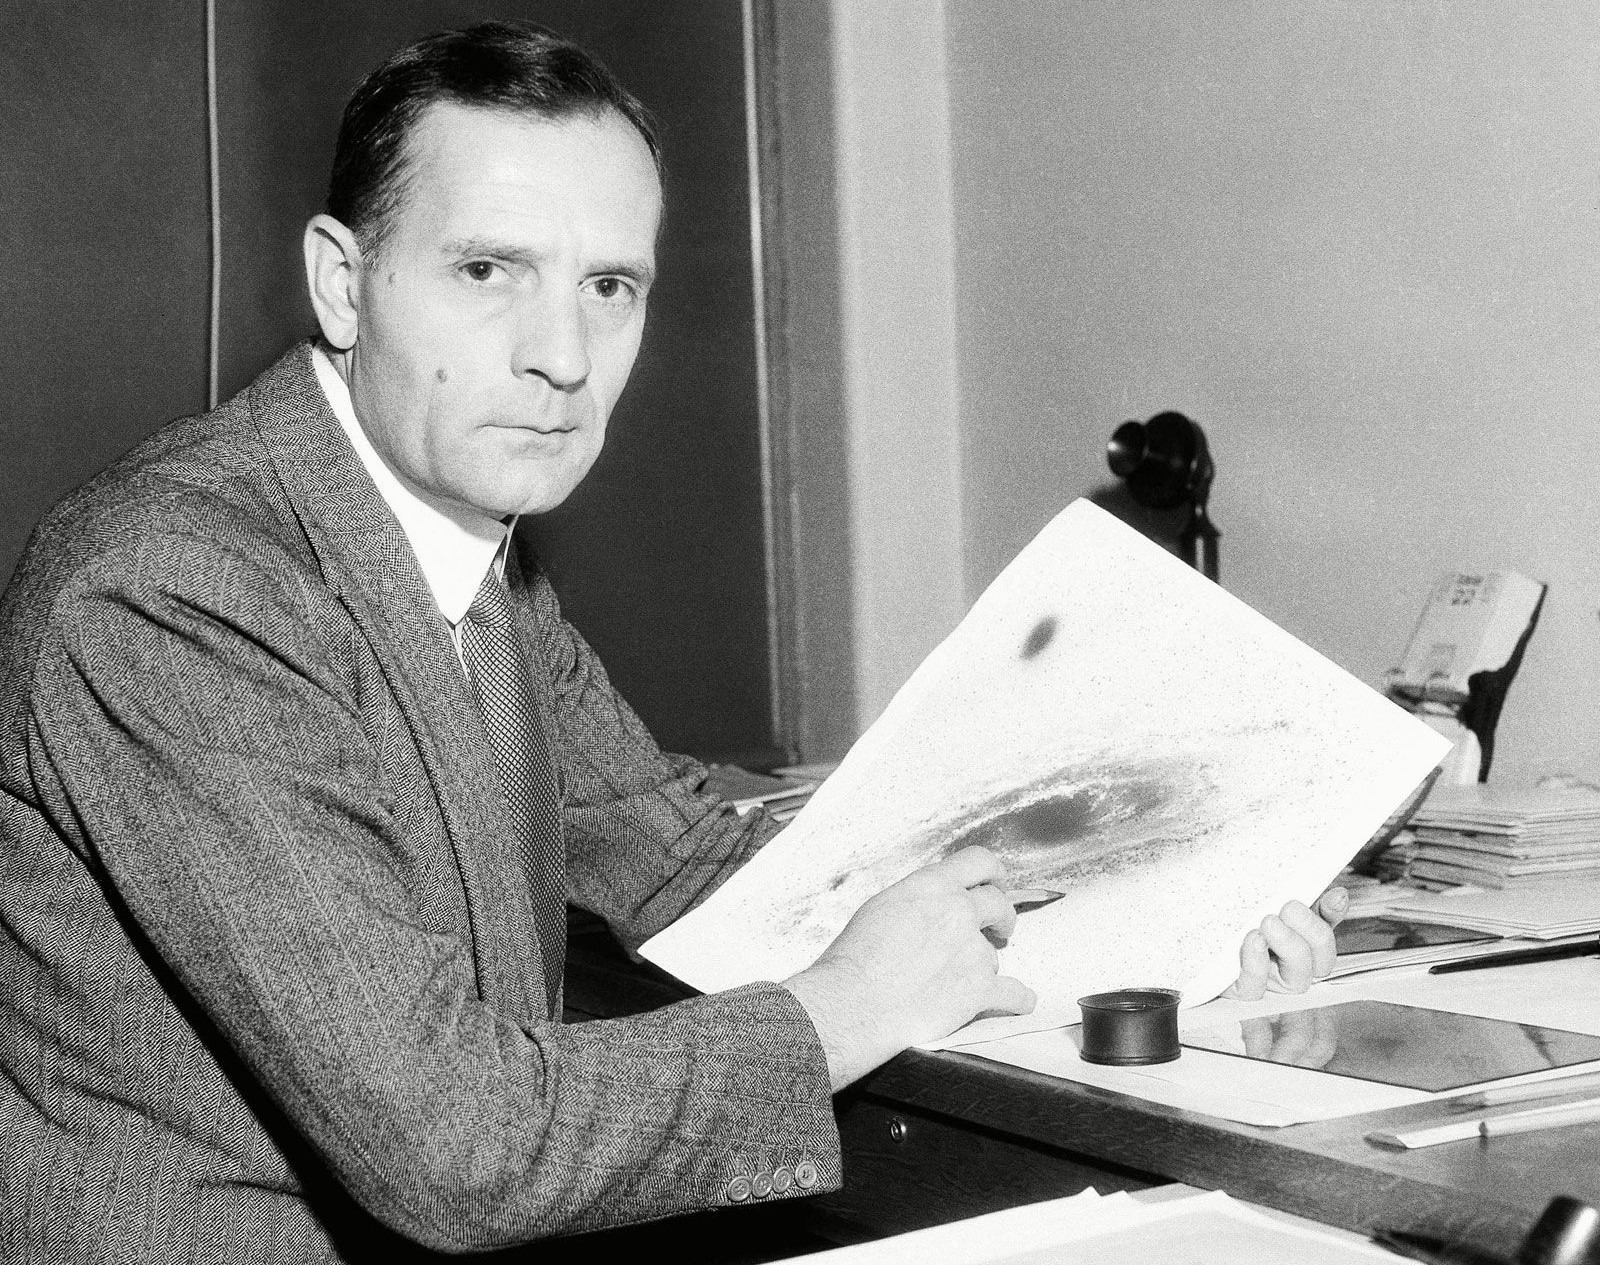
\includegraphics[width= 1\linewidth]{9}
		\caption{\small\textit{\color{timhieukhoahoc}Edwin Hubble $(1889 - 1953)$.}}
		\vspace*{-10pt}
	\end{figure}
	Năm $1921$, Shapley trở thành giám đốc của đâì thiên văn Havard, thay cho Pickering đã qua đời một năm trước. Shapley muốn Leavitt tiến hành sâu hơn các phân tích về các sao biến quang, công việc mà Leavitt đã không có thời gian theo đuổi do phải thực hiện một số dự án khác mà Pickering cho là quan trọng hơn. Tuy nhiên, mọi việc đã không diễn ra như mong đợi. Leavitt bị mắc bệnh ung thư và qua đời vào tháng $11$ năm $1921$.
	\begin{figure}[H]
		\vspace*{-5pt}
		\centering
		\captionsetup{labelformat= empty, justification=centering}
		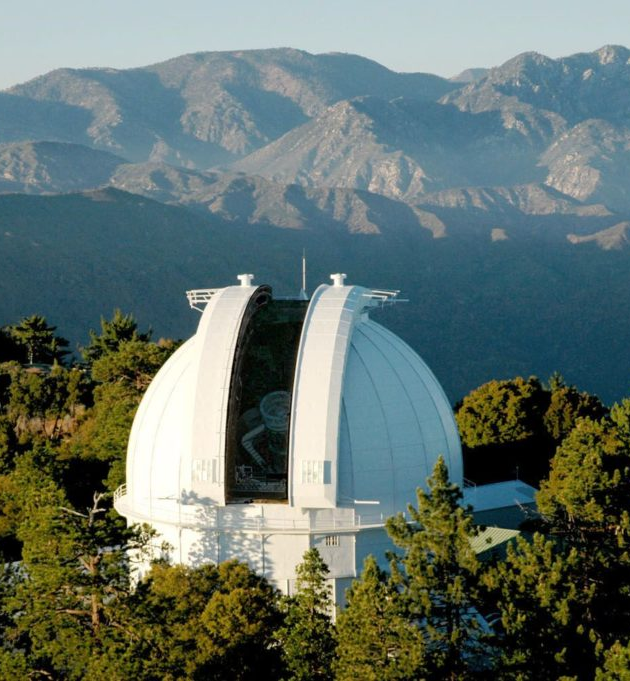
\includegraphics[width= 1\linewidth]{10}
		\caption{\small\textit{\color{timhieukhoahoc}Hình $7$. Đài thiên văn trên núi Wilson với kính viễn vọng $100$ inch mà Hubble đã sử dụng.}}
		\vspace*{-10pt}
	\end{figure}
	Trong khi Shapley vẫn tiếp tục cuộc tranh cãi học thuật về các kết quả của mình thì Hubble lại cần mẫn hướng kính viễn vọng lên bầu trời ở đỉnh núi Wilson để tìm dữ liệu mới có thể mang đến đột phá. Tháng 10 năm 1923, khi quan sát các nova trong tinh vân Andromeda, Hubble đã phát hiện ra một ngôi sao Cepheid. Từ chu kỳ của ngôi sao này, theo công thức của Leavitt đã được Shapley bổ sung các hệ số, ông tính ra được khoảng cách từ tinh vân Andromeda đến Trái Đất là $1$ triệu năm ánh sáng (con số hiện nay là hơn $2$ triệu năm ánh sáng do việc ánh sáng bị hấp thụ trên đường truyền đã không được Hubble xét đến)!  Tiếp tục vài tháng sau, ông lại tìm ra một Cepheid nữa cùng nhiều nova khác.
	\vskip 0.1cm
	Với những số liệu chắc chắn, Hubble gửi bức thư kèm theo các biểu đồ cho Shapley để thông báo kết quả. Sự kiện này đánh dấu thời điểm mô hình vũ trụ của Shapley đã sụp đổ. Trong khoảng thời gian tiếp theo, Hubble còn tìm thấy theo nhiều Cepheid trong tinh vân Andromeda cũng như một thiên hà khác cách Trái Đất $700000$ năm ánh sáng. Hubble báo cáo kết quả của mình trước các nhà khoa học khác năm $1925$ và công bố bài báo khoa học năm $1929$. Đến đây thì hầu như tất cả mọi người đều đã hiểu, dải Ngân hà của chúng ta chỉ là một thiên hà trong rất nhiều thiên hà khác của vũ trụ này.
	\begin{figure}[H]
		\vspace*{-5pt}
		\centering
		\captionsetup{labelformat= empty, justification=centering}
		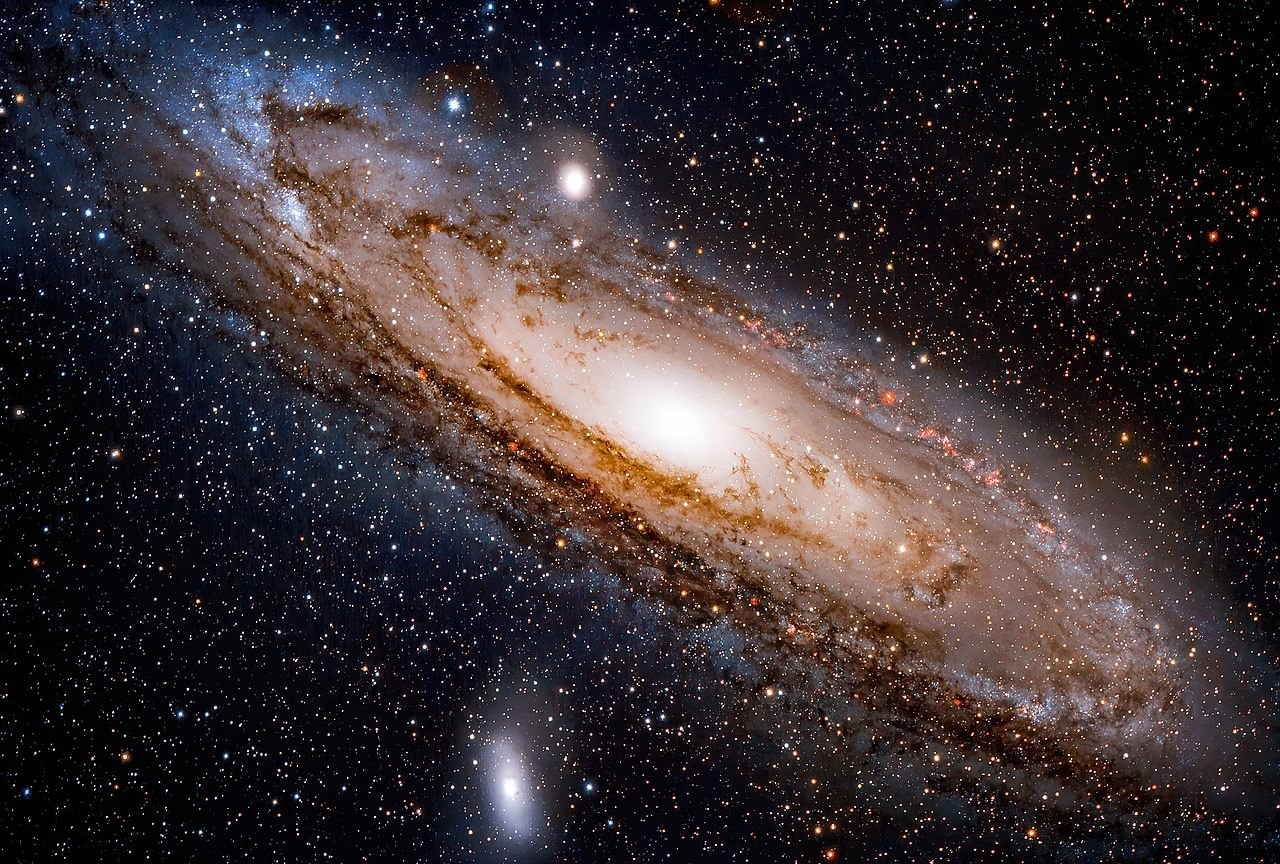
\includegraphics[width= 1\linewidth]{11}
		\caption{\small\textit{\color{timhieukhoahoc}Hình $8$. Ảnh chụp của tinh vân Andromeda cho thấy nó là thiên hà với nhiều hệ Mặt Trời.}}
		\vspace*{-10pt}
	\end{figure}
	Không dừng lại ở đây, Hubble bắt đầu nghiên cứu mối liên hệ giữa khoảng cách từ các thiên hà đến Trái Đất và vận tốc của chúng. Vận tốc di chuyển của mỗi thiên hà có thể được xác định nhờ quang phổ mà ta quan sát được từ thiên hà đó. Do hiệu ứng Doppler, các vật thể chuyển động hướng về Trái Đất (như tinh vân Andromeda) có quang phổ lệch về phía bước sóng xanh (blueshift) trong khi các thiên hà khác rời ra xa Trái Đất sẽ có quang phổ lệch về phía bước sóng đỏ (redshift). Vận tốc di chuyển càng lớn sẽ cho độ lệch càng lớn. Với những thiên hà có các ngôi sao Cepheid quan sát được, Hubble thấy quan hệ tuyến tính giữa vận tốc đo bằng quang phổ và khoảng cách tới Trái Đất xác định theo chu kỳ của các sao Cepheid. Hằng số tỷ lệ giữa vận tốc và khoảng cách này hiện nay được gọi là hằng số Hubble. Sử dụng mối quan hệ tuyến tính vừa mới tìm ra, Hubble dùng các độ lệch sang bước sóng đỏ để tìm cả khoảng cách lẫn vận tốc của các thiên hà ở quá xa mà ta không thể quan sát được các sao Cepheid của chúng. Hubble cho ra hình ảnh của một vũ trụ mới, không chỉ rất rộng lớn và mà còn đang chuyển động. Những thiên hà ở càng xa thì càng chuyển động ra xa ta với vận tốc lớn hơn. Phát hiện của Hubble cũng giúp Albert Einstein hoàn thiện thuyết tương đối. Trước đó, các phương trình của ông cho thấy vũ trụ có kích thước không gian thay đổi. Tin tưởng rằng không gian là cố định, Einstein đã thêm vào một ``hằng số vũ trụ"  để loại trừ ảnh hưởng của trọng lực nhằm dẫn đến một vũ trụ tĩnh. Sau khi biết kết quả của Hubble, Einstein đã gọi hằng số vũ trụ này là sai lầm khoa học lớn nhất của mình và sửa lại các công thức của thuyết tương đối.
	\vskip 0.1cm
	Một vấn đề được đặt ra khi biết vũ trụ vẫn đang dãn nở là nếu đi ngược thời gian, vũ trụ sẽ nhỏ dần lại. Vậy có phải ở một thời điểm nào đó, vũ trụ này chỉ là một điểm?  Đây cũng là cơ sở của thuyết ``big bang" về sự ra đời của vũ trụ. Cho đến ngày nay, sự thực về nguồn gốc và quá trình hình thành của vũ trụ vẫn còn là một câu hỏi lớn của khoa học với nhiều vấn đề còn bỏ ngỏ.
	\vskip 0.1cm
	$\pmb{4.}$ \textbf{\color{timhieukhoahoc}Lời kết}
	\vskip 0.1cm
	Ảnh hưởng của Leavitt đến sự phát triển của thiên văn học có thể nói là rất to lớn. Năm $1924$, nhà toán học Thụy Điển  Gustaf Mittag--Leffler đề cử bà cho giải Nobel mà không biết rằng Leavitt đã mất từ vài năm trước đó. Những đóng góp của Leavitt cùng các ``computer" khác tại đài thiên văn Havard hầu như chỉ xuất hiện ở các chú thích trong giáo trình thiên văn. Sự cống hiến của họ cho khoa học thật sự xứng đáng được công chúng biết đến nhiều hơn nữa.
	\begin{figure}[H]
		\vspace*{-5pt}
		\centering
		\captionsetup{labelformat= empty, justification=centering}
		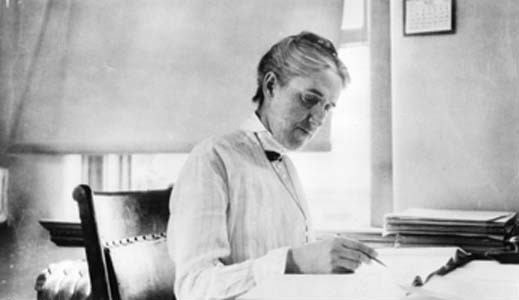
\includegraphics[width= 1\linewidth]{12}
		\caption{\small\textit{\color{timhieukhoahoc}Leavitt khi làm việc tại đài thiên văn Havard}}
		\vspace*{-10pt}
	\end{figure}
	\textbf{\color{timhieukhoahoc}Tài liệu tham khảo}
	\vskip 0.1cm
	[$1$] Fernie, J. D. ($1969$). The Period--Luminosity Relation: A Historical Review. \textit{Publications of the Astronomical Society of the Pacific}, $81$, $707$. \url{https://doi.org/10.1086/128847}
	\vskip 0.1cm
	[$2$] Johnson, G. ($2006$).  . W.W. Norton.
	\vskip 0.1cm
	[$3$] Trimble, V. ($1995$). The $1920$ Shapley--Curtis Discussion: Background, Issues, and Aftermath. \textit{Publications of the Astronomical Society of the Pacific}, $107$, $1133$. \url{https://doi.org/10.1086/133671}
\end{multicols}


